\documentclass[tikz]{standalone}

\usetikzlibrary{shapes.arrows}

\begin{document}
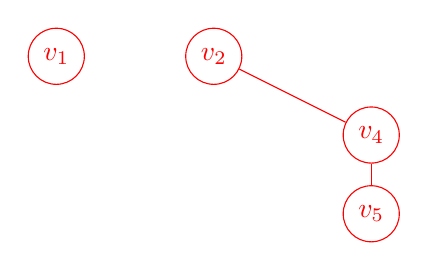
\begin{tikzpicture}[every node/.style={circle, draw}]
    \node[red] (v1) at (0, 0) {$v_1$};
    \node[red] (v2) at (2, 0) {$v_2$};
    \node[red] (v4) at (4, -1) {$v_4$};
    \node[red] (v5) at (4, -2) {$v_5$};

    \draw[red] (v2) -- (v4);
    \draw[red] (v4) -- (v5);
\end{tikzpicture}
\end{document}